
\section{Undersökningsmetoder}
Detta kapitel beskriver vilka metoder som använts i undersökningen. Metoderna är
valda och specifierade så att de skall kunna ge svar på ett antal följdfrågor som
identifierats i denna undersökning. Först anges frågorna och sedan följer
metodbeskrivning.

\subsection{Frågor att besvara i undersökningen}
Frågorna kategoriseras i följande kategorier... (eventuellt)
\begin{enumerate}
    \item Hur skall man bedöma/redovisa om en delprojektmetod eller praktik är bra?
    \item Hur kan man kategorisera, välja och namnge projektmetoder (projektpraktiker)
    och (verklighetsbeskrivning) så att diskussionen om dito blir begreppsmässigt
    konsistent för ingenjörer inom IT-området (s.k. ontologi?).
    \item Vilka ansvarsroller skall användas som ansats i projektet?
    \item Vad består ett projekt av och vilka metoder/praxis skall användas, undersökas
    och bedömas? Vilken ansats skall göras?
    \item (Vad och hur skall eller behöver jag som student redovisa i rapporten för att
    bli godkänd på kursen? Denna fråga tas bort i den slutliga rapporten)
\end{enumerate}

\subsection{Metodbeskrivning (undersökningsmetod)}
Den centrala metoden i undersökningen är att avgöra om olika valda projekt-praktiker 
och arbetssätt är ”bra” och om de bidrar till att göra hela projektprocessen bra. 
Åstadkommer/skapar projektet rätt saker och konstrueras lösningar på bästa sätt? 
Metoden för att samla data i denna fråga blir induktiv då erfarenheten i gruppen är 
ytterst liten. Arbetssättet blir att efterhand som projektet fortskrider så förs 
bedömningsområden som anses vitala och bedömningskriterier in i en tabell kontinuerligt. 
Tabellen, se kapitel ”Resultat”, dess innehåll och dess utformning förbättras också hela 
tiden.\\

\textbf{Metod 1: Undersökningsmetod}, se figur nrX. De gula fälten är aktiviteter som 
kopplar till själva undersökningen. Metoden följer principer för vetenskaplighet 
enligt Andersson och Ekholm.
 
\begin{figure}[htbp]
    \centerline{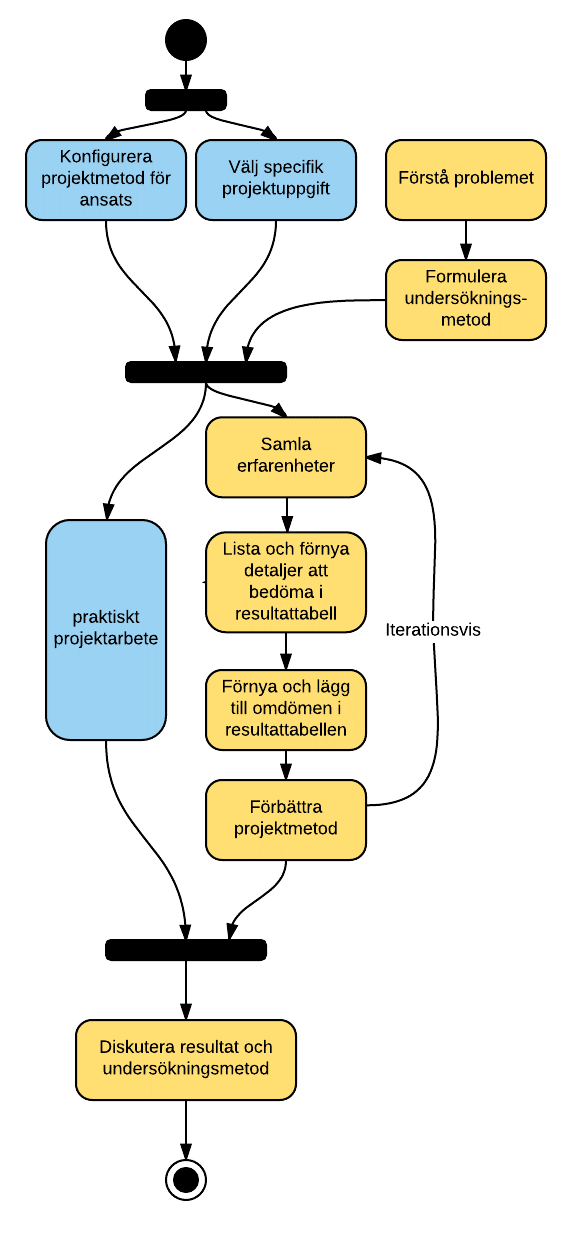
\includegraphics[max height=250px, max width=250px]{images/undersokningsmetod.png}}
    \caption{Undersökningsmetod för "Vad är bra projektmetod för små IT-projekt"}
    \label{fig}
\end{figure}

\textbf{Metod 2: Begrepp}
Begrepp som används följer om möjligt OMGs standard 
\textit{Essence - Kernel and Language for Software Engineering Methods Version 1.0}.

Följande bilder listar illustrativt centrala begrepp. I denna artikel kommer de engelska
begreppen att fritt översättas till svenska då risken för missförstånd anses liten.

\begin{figure}[htbp]
    \centerline{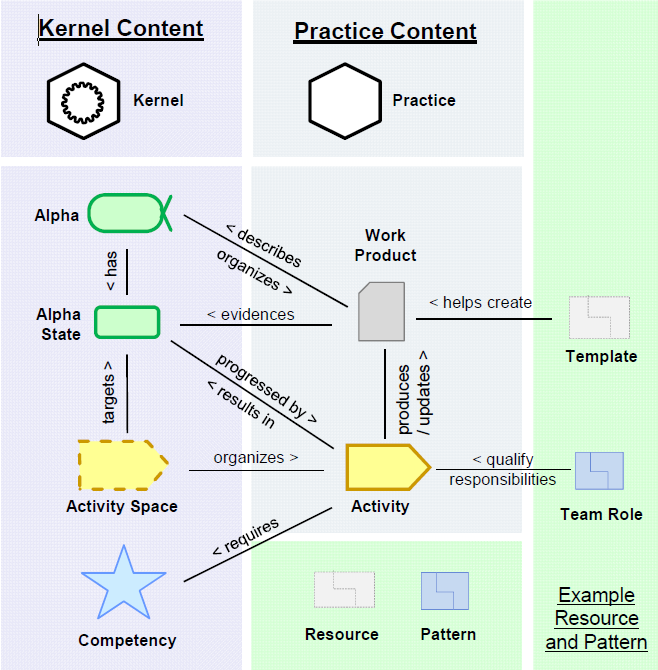
\includegraphics[max height=250px, max width=250px]{images/begrepp.png}}
    \caption{Begrepp}
    \label{fig}
\end{figure}

\begin{figure}[htbp]
    \centerline{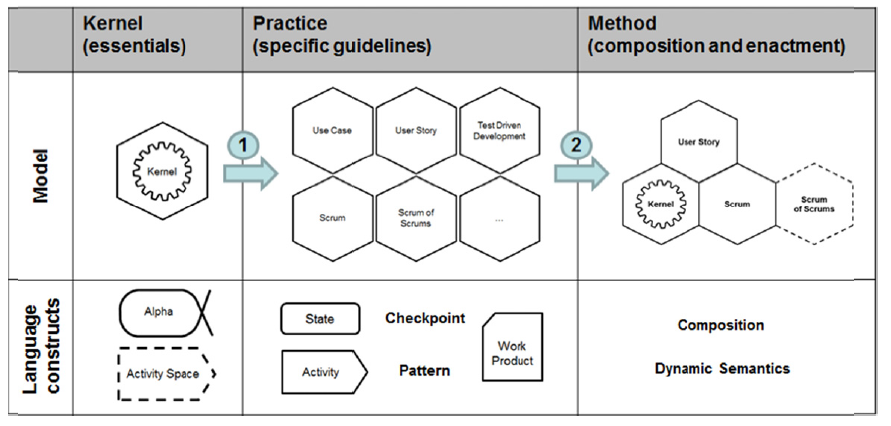
\includegraphics[max height=250px, max width=250px]{images/practicemethod.png}}
    \caption{Practice and Method}
    \label{fig}
\end{figure}